% 3.1.PrepareApplication.tex
%	Last update: 2019/10/03 F.Kanehori
%\newpage
\subsection{sByVELhUuWQYiYYM}
\label{subsec:PrepareApplication}

\noindent
\KLUDGE アプリケーションと並行してSpringhead\KLUDGE ライブラリを開発する場合には、
\KQuoteS\ref{subsec:Problems} CMake\KLUDGE を使用した場合の問題点\KQuoteE
\KLUDGE で示した問題に対処する必要があるため、
\KLUDGE ここで述べる方法に従って作業を進めてください
(\KQuote{\ref{subsec:Solution} \KLUDGE 対処法}\KLUDGE で示した方策が組み込まれます)\KLUDGE 。

\medskip
\KLUDGE 以下、Springhead\KLUDGE ライブラリをダウンロードしたディレクトリを\SprTop{} \KLUDGE 、
\KLUDGE アプリケーションプログラムを作成するディレクトリを\AppTop{}\KLUDGE として説明を進めます。

\bigskip
\noindent
\AppTop{}\KLUDGE に移動してください。

\bigskip
\noindent
\KLUDGE 配布されたファイル\CMakeTopdir{.dist}\KLUDGE を\CMakeTopdir{}\KLUDGE という名前で、
\CMakeLists{.Dev.dist}\KLUDGE を\CMakeLists{}\KLUDGE という名前でコピーします
(\KLUDGE 誤ってコミットするのを防ぐためにも、リネームではなくコピーしてください)。

\medskip
\ifLwarp
	\begin{figure}[h]
	    \begin{center}
	    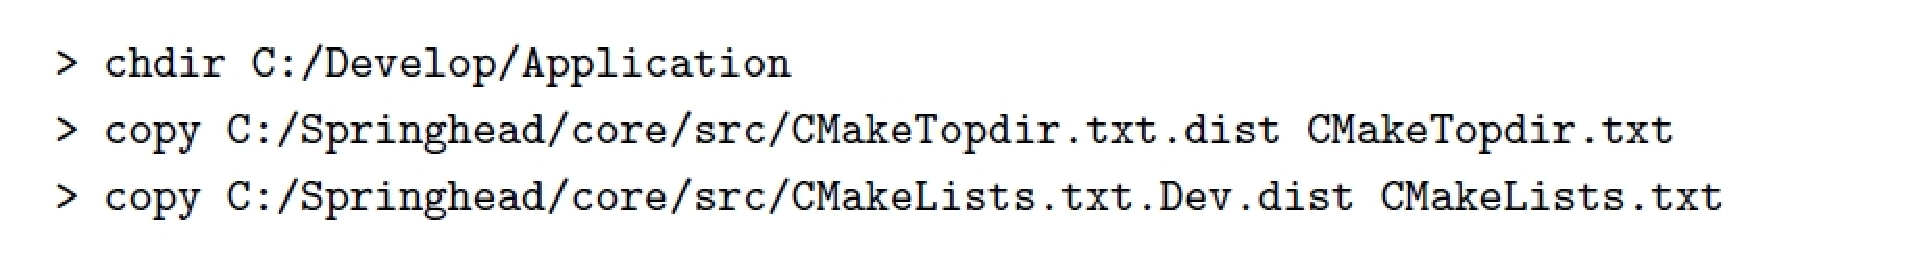
\includegraphics[width=\textwidth]{fig/command-3-1-a.eps}
	    \end{center}
	    \label{fig:DownloadTree}
	\end{figure}
\else
\begin{narrow}[15pt]
	\CmndBox{%
	{\small{\textgreater  chdir C:/Develop/Application}}\\
	{\small{\textgreater  copy C:/Springhead/core/src/CMakeTopdir.txt.dist CMakeTopdir.txt}}\\
	{\small{\textgreater  copy C:/Springhead/core/src/CMakeLists.txt.Dev.dist CMakeLists.txt}}
	}
\end{narrow}
\fi

\bigskip
\noindent
\bf{\CMakeTopdir{}}\KLUDGE の編集
\begin{narrow}[20pt]
	\SprLib \KLUDGE をダウンロードしたディレクトリを\CMakeTopdir{}\KLUDGE には\SprLib \KLUDGE に設定します。
	\KLUDGE これは、CMake\KLUDGE にSpringhead\KLUDGE のソースツリーの場所を教えるために必要な設定です。

\ifLwarp
	\begin{figure}[h]
	    \begin{center}
	    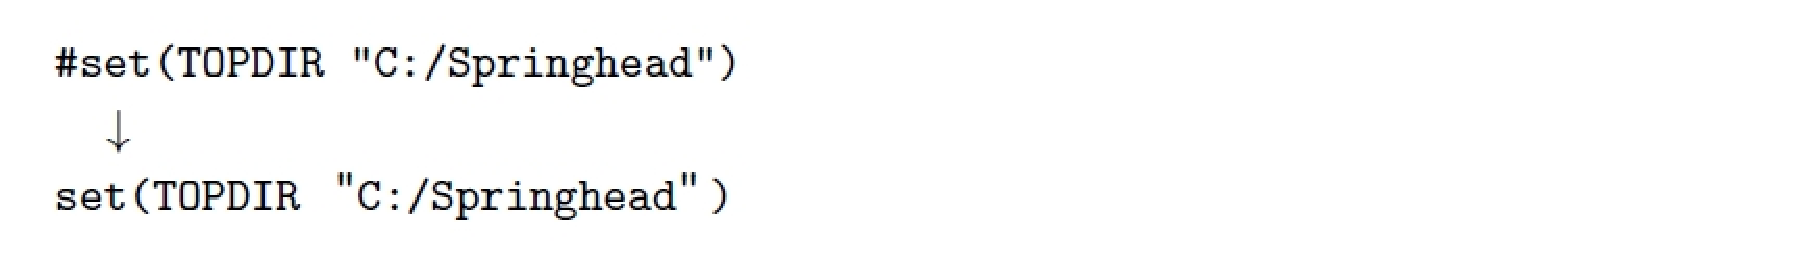
\includegraphics[width=\textwidth]{fig/command-3-1-b.eps}
	    \end{center}
	    \label{fig:DownloadTree}
	\end{figure}
\else
	\begin{narrow}[15pt]
		\CmndBox{%
			{\small{=ESCAPEx23=set(TOPDIR "C:/Springhead")}}\\
			\hspace{10pt}{\small{$\downarrow$}}\\
			{\small{set(TOPDIR \SprTop{})}}
		}
	\end{narrow}
\fi
\end{narrow}
\medskip
\noindent
\bf{\CMakeLists{}}\KLUDGE の編集
\begin{narrow}[20pt]
	\begin{enumerate}
	    \item
		\KLUDGE プロジェクト名を設定します(11\KLUDGE 行目)\KLUDGE 。

\ifLwarp
		\begin{figure}[h]
			\begin{center}
			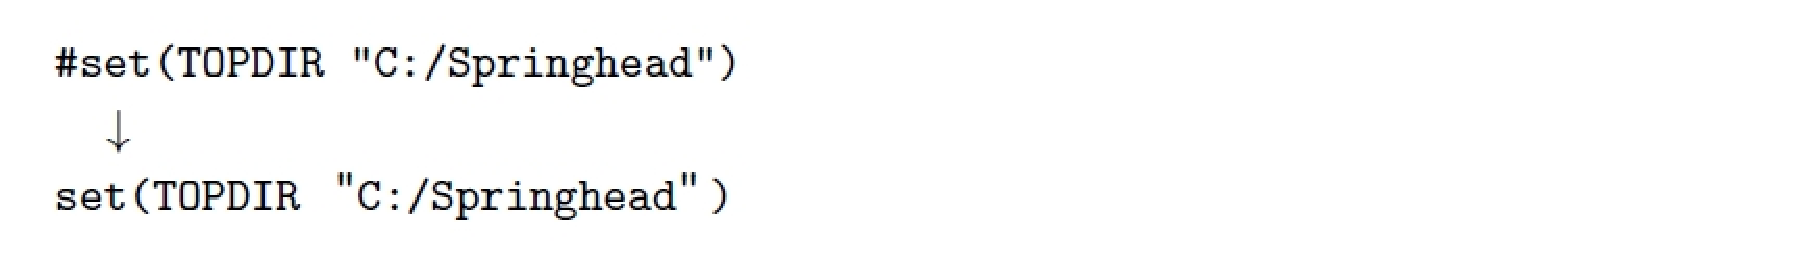
\includegraphics[width=\textwidth]{fig/command-3-1-b.eps}
				\end{center}
			\label{fig:DownloadTree}
		\end{figure}
\else
		\begin{narrow}[s][5pt]
			\CmndBox{%
				{\small{set(ProjectName "Project")}}\\
				\hspace{10pt}{\small{$\downarrow$}}\\
				{\small{set(ProjectName "\textless \it{MyApplication}\textgreater ")}}
			}
		\end{narrow}
		\Vskip{.5\baselineskip}
\fi

	    \item
		Customization section (19\KLUDGE 行目以降)\KLUDGE を必要に応じて変更します。\\
		\KLUDGE 各変数の意味は次のとおりです。

		\medskip
		\def\SetRelPath{\tt{RELATIVE \$\{CMAKE\_SOURCE\_DIR\}}}
		\def\CMakeSrcDir{\tt{\$\{CMAKE\_SOURCE\_DIR\}}}
		\def\Explanation=ESCAPEx23=1{\begin{minipage}[t]{222pt}{=ESCAPEx23=1}\end{minipage}}

		\begin{narrow}[4pt]
		\begin{tabular}{|l|l|}\hline
		    \tt{OOS\_BLD\_DIR} &
			%\begin{minipage}[t]{220pt}
			%CMake\KLUDGE の作業領域(\KLUDGE ディレクトリ)\KLUDGE の名前(\KLUDGE 本ドキュメントで
			%\build \KLUDGE としているもの)\KLUDGE 。
			%\end{minipage}
			%\\\hline
			CMake\KLUDGE の作業領域(\KLUDGE ディレクトリ)\KLUDGE の名前(\KLUDGE 本ドキュ\\
			& \KLUDGE メントで\build \KLUDGE としているもの)\KLUDGE 。\\\hline
		    \multicolumn{2}{|l|}{%
			\tt{CMAKE\_CONFIGURATION\_TYPES}} \\
			& \KLUDGE ビルド構成。\\\hline
		    \tt{SRCS} &
			\KLUDGE ビルドの対象とするファイル。
			\KLUDGE 設定は\tt{set(SRCS \KLUDGE …)} \\
			& \KLUDGE または\tt{file(GLOB SRCS \KLUDGE …)}\KLUDGE とします。\\
			& \KLUDGE 後者ではワイルドカードが使えます。\\
			& \tt{SRCS}\KLUDGE の直後に``\tt{RELATIVE \textless \it{base-dir}\textgreater }''\KLUDGE を付加すると \\
			& \KLUDGE 相対パス指定となります。デフォルトは \\
			& \ \ {\footnotesize{\tt{file(GLOB \SetRelPath\ *.cpp *.h)}}} \\
			& \KLUDGE です。\\\hline
		    \tt{EXCLUDE\_SRCS} &
			\KLUDGE ビルドの対象から外すファイル。\\
			& \KLUDGE 上の\tt{SRCS}\KLUDGE で\tt{RELATIVE}\KLUDGE としていないときは絶対パス \\
			& \KLUDGE で指定します。\\
			& \tt{SRCS}\KLUDGE でワイルドカードを使用した場合に有用です。\\\hline
		    \tt{SPR\_PROJS} &
			\KLUDGE アプリケーションに組み込むSpringhead\KLUDGE ライブラリ\\
			& \KLUDGE のプロジェクト名。\\
			& \KLUDGE 不要なプロジェクト名を削除します。
			\KLUDGE この中にRun-\\
			& Swig\KLUDGE を含めてはいけません。\\\hline
		    \tt{ADDITIONAL\_INCDIR} &
			\KLUDGE 追加のインクルードパス指定。\\
			& \KLUDGE 現在のディレクトリは \CMakeSrcDir \KLUDGE で参照 \\
			& \KLUDGE できます。\\\hline
		    \tt{ADDITIONAL\_LIBDIR} &
			\KLUDGE 追加のライブラリパス指定。\\\hline
		    \tt{ADDITIONAL\_LIBS} &
			\KLUDGE 追加のライブラリファイル名。\\\hline
		    \tt{EXCLUDE\_LIBS} &
			link\KLUDGE の対象から外すライブラリファイル名。\\
			& \KLUDGE デフォルトで組み込まれてしまうライブラリファイル\\
			& \KLUDGE を排除するために指定します。\\\hline
\ifLwarp\else
		\end{tabular}
		\begin{tabular}{|l|l|}\hline
\fi
		    \multicolumn{2}{|l|}{%
			\tt{DEBUGGER\_WORKING\_DIRECTORY}} \\
			\phantom{\tt{ADDITIONAL\_INCDIR}}
			& Visual Studio Debugger\KLUDGE の作業ディレクトリ名。\\
			& \KLUDGE デバッガはこのディレクトリで起動されたように振る \\
			& \KLUDGE 舞います。\\\hline
		    \multicolumn{2}{|l|}{%
			\tt{DEBUGGER\_COMMAND\_ARGUMENTS}} \\
			& Visual Studio Debugger\KLUDGE に渡すコマンド引数 \\\hline
		\end{tabular}
		\end{narrow}
	\end{enumerate}
\end{narrow}

\bigskip
\noindent
\KLUDGE 自前でインストールしているパッケージ
(\tt{boost}, \tt{glew}, \tt{freeglut}, \tt{glui})\KLUDGE を使用する場合には、
\KLUDGE さらに、
\KLUDGE 配布されたファイル\CMakeConf{.dist}\KLUDGE を\CMakeConf{}\KLUDGE という名前でコピーして
\KLUDGE 必要な編集をします。
\KQuote{\ref{subsec:PrepareLibrary} \KLUDGE 準備}\KLUDGE を参照してください。

\medskip
\noindent
\KLUDGE ビルドの条件(compile/link\KLUDGE のパラメータ)\KLUDGE を変更したいときは、
\KLUDGE 配布されたファイル\CMakeOpts{.dist}\KLUDGE を\CMakeOpts{}\KLUDGE という名前でコピーして
\KLUDGE 適宜変更してください。

\medskip
\noindent
\KLUDGE 以上で準備作業は終了です。

% end: 3.1.PrepareApplication.tex
